\chapter{Forward and Inverse Kinematics}\label{chap:kinematics}
In order to plan a robot's movements, we have to understand the relationship between the actuators that we can control and the robot's resulting position in the environment. For static arms, this is rather straightforward: if we know the position/angle of each joint, we can calculate the position of its end-effectors using trigonometry. This process is known as \emph{forward kinematics}. \index{Forward Kinematics} If we want to calculate the position each joint needs to be at, we need to invert this relationship. This is known as inverse kinematics. \index{Inverse Kinematics}

The goals of this chapter are:

\begin{itemize}
\item introduce coordinate systems and their transformations,
\item to introduce the forward kinematics of mobile robots and simple arms,
\item show how solutions for the inverse kinematics for both static and mobile robots can be derived,
\item provide an intuition on the relationship between inverse kinematics and path-planning.
\end{itemize}

\section{Coordinate Systems and Frames of Reference}\label{sec:coordsystems}
Every robot assumes a position in the real world that can be described by its position (x, y and z) and orientation (pitch, yaw and roll) along the three major axes of a Cartesian Coordinate system (See also Section \ref{sec:dof}, ``Degrees of freedom''). Such a coordinate system is shown in Figure \ref{fig:coordinatesystem}. Note that the directions and orientations of the coordinate axes are arbitrary. This books uses the ``right hand rules'', which is illustrated in Figure \ref{fig:coordinatesystem} to determine axes labels and directions throughout.

\begin{figure}
	\centering
		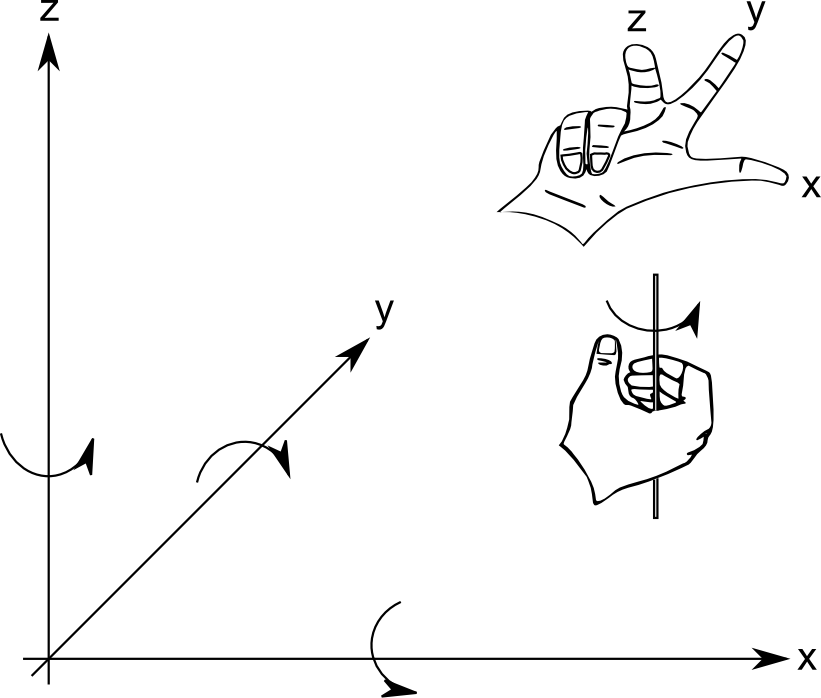
\includegraphics[width=0.8\textwidth]{figs/coordinatesystem.png}
	\caption{A coordinate system indicating the direction of the coordinate axes and rotation around them. These directions have been derived using the right-hand rules.}
	\label{fig:coordinatesystem}
\end{figure}

Defining all three position axes and orientations might be cumbersome. What level of detail we care about, where the origin of this coordinate system is, and even what kind of coordinate system we chose, depends on the specific application. For example, a simple mobile robot would typically require a representation with respect to a room, a building, or the earth's coordinate system (given by the longitude and latitude of each point on the earth), whereas a static manipulator usually has the origin of its coordinate system at it's base. More complicated systems, such as mobile manipulators or multi-legged robots, make live much easier by defining multiple coordinate systems, e.g.\ one for each leg and one that describes the position of the robot in the world frame. These local coordinate systems are known as \emph{Frame of Reference}\index{Frame of Reference}. An example of two nested coordinate systems is shown in Figure \ref{fig:for}. In this example, a robot located at the origin of $x',y'$ and $z'$ might plan its motions in its own reference frame, which can then be expressed in the coordinate system $x$, $y$ and $z$ by performing a translation and a rotation as we will later see. 

Depending on it's degrees-of-freedom, that is the number of independent translations and rotations a robot can achieve in Cartesian space, it is also customary to ignore components of position and orientation that remain constant. For example a simple floor-cleaning robot's pose might be completely defined by it's $x$ and $y$ coordinates in a room as well as its orientation, i.e.\ its rotation around the $z$-axis. 


\begin{figure}
	\centering
		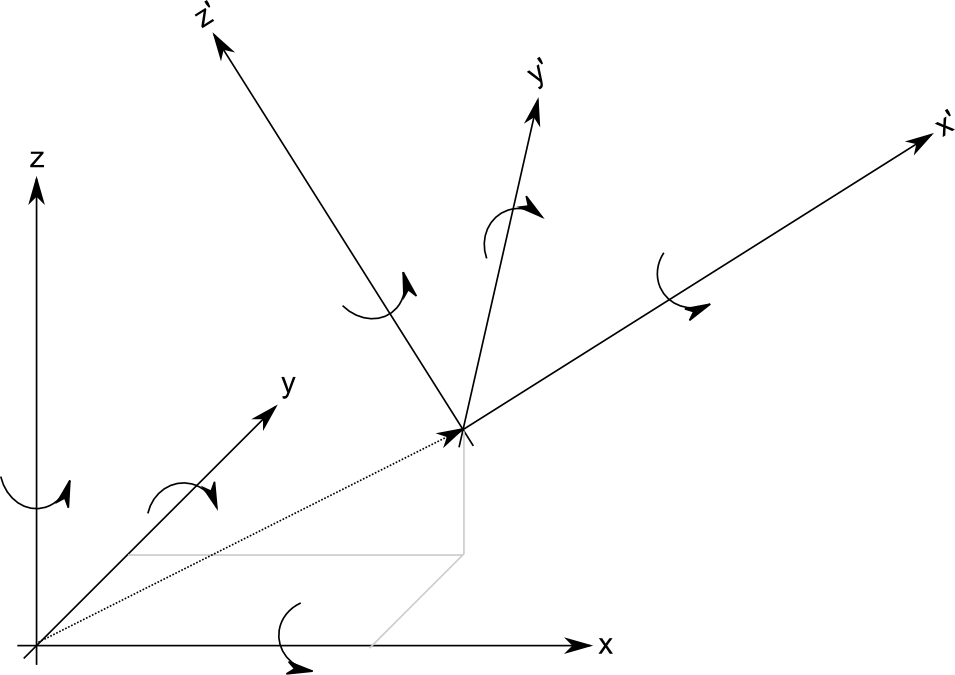
\includegraphics[width=\textwidth]{figs/frameofreference.png}
	\caption{Two nested coordinate systems (frames of reference).}
	\label{fig:for}
\end{figure}

\subsection{Matrix notation}
Given some kind of fixed coordinate system, we can describe the \emph{position} of a robot's end-effector by a $3x1$ position vector. As there can be many coordinate systems defined on a robot and the environment, we identify the coordinate system a point relates to by a preceeding super-script, e.g., $ ^AP$ to indicate that point $P$ is in coordinate system $\{A\}$. Each point consists of three elements $ ^AP=[p_x p_y p_z]^T$.

As we know, not only the position of the robot is important, but also its orientation. In order to describe the orientation of a point, we will attach a coordinate system to it. Let $ \hat{X}_B, \hat{Y}_B$ and $ \hat{Z}_B$ be unit vectors that correspond to the principal axes of a coordinate system $\{B\}$. When expressed in coordinate system $\{A\}$, they are denoted $^A\hat{X}_B, ^A\hat{Y}_B$ and $ ^A\hat{Z}_B$. In order to express a vector that is given in one coordinate system in another, we need to project each of its components to the unit vectors that span the target coordinate system. For example

\begin{equation}\label{eq:projection}
^A\hat{X}_B=(\hat{X}_B\cdot\hat{X}_A, \hat{X}_B\cdot\hat{Y}_A,\hat{X}_B\cdot\hat{Z}_A)^T
\end{equation}
consists of the projections of $\hat{X}_B$ onto $\hat{X}_A$, $\hat{Y}_A$ and $\hat{Z}_A$. Here,  $|\cdot|$ denotes the scalar product (also known as dot or inner product).  Note that all vectors in (\ref{eq:projection}) are unit vectors, i.e. their length is one. By definition of the scalar product, $A\cdot B=\|A\|\|B\|\cos \alpha=\cos \alpha$, indeed reduces the projection of $\hat{X}_B$ onto the unit vectors of $\{A\}$. This projection is illustrated in Figure \ref{fig:projection}.

\begin{figure}
	\centering
		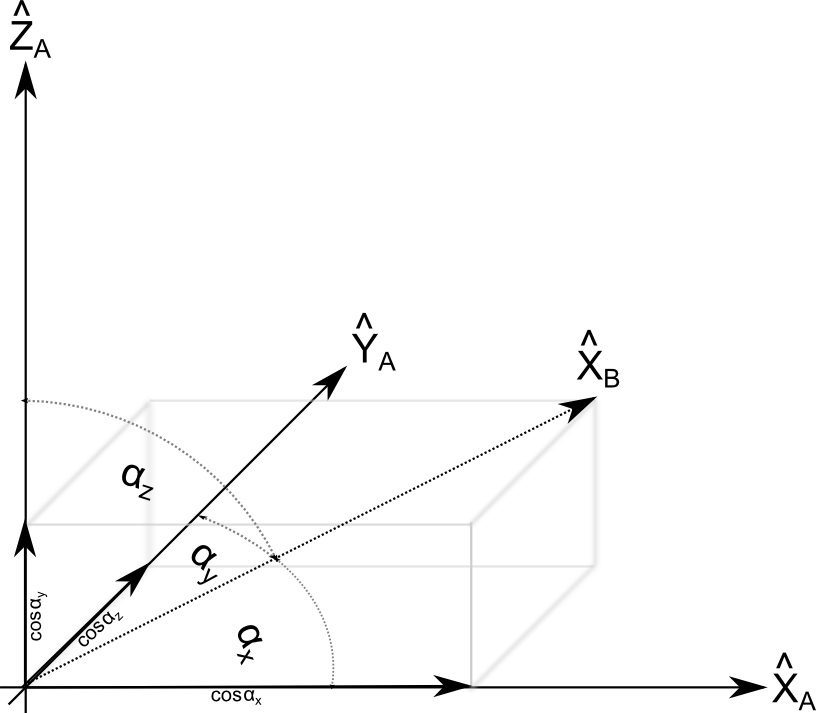
\includegraphics[width=\textwidth]{figs/projection.png}
	\caption{The projection of the unit vector $\hat{X}_B$ onto the unit vectors that span coordinate system $\{A\}$. As all vectors are unit vectors, $A\cdot B=\|A\|\|B\|\cos \alpha=\cos \alpha$. For clarity, only $\hat{X}_B$ of coordinate system $\{B\}$ is shown. }
	\label{fig:for}
\end{figure}

We can now do this for all three vectors that span coordinate system $\{B\}$ and stack these three vectors together into a 3x3 matrix to obtain the rotation matrix
%
\begin{equation}
^A_BR=[^A\hat{X}_B ^A\hat{Y}_B ^A\hat{Z}_B]
\end{equation}
%
which describes $\{B\}$ relative to $\{A\}$. It is important to note that all columns in $ ^A_BR$ are unit vectors, so that the rotation matrix is orthogonal. This is important as this allows us to easily obtain the inverse of $ ^A_BR$ as $ ^A_BR^T$ or
$ ^B_AR=^A_BR^T$. 

%http://www.youtube.com/watch?v=CxsF2xV78RQ

We have now established how to express the orientation of a coordinate system using a rotation matrix. Usually, coordinate systems don't lie on top of each other, but are also displaced from each other. 
Together, position and orientation is known as a \emph{frame},\index{Frame} which is a set of four vectors, one for the position and three for the orientation, and we can write
%
\begin{equation}
\{B\}=\{^A_BR, ^AP\}
\end{equation}
%
to describe the coordinate frame $\{B\}$ with respect to $\{A\}$ using a vector $^AP$ and a rotation matrix $^A_BR$. Robots usually have many such frames defined along their bodies.

\subsection{Mapping from one frame to another}
Having introduced the concept of frames, we need the ability to map coordinates in one frame to coordinates in another frame. For example, lets consider frame $\{B\}$ having the same orientation as frame $\{A\}$ and sitting at location $^AP$ in space. As the orientation of both frames is the same, we can express a point $ ^BQ$ in frame $\{A\}$ as
%
\begin{equation}
^AQ=^BQ+^AP
\end{equation}
%
Actually, adding two vectors that are in different reference frames, i.e., $ ^BQ+^AP$, is only possible if both of them have the same orientation. We can, however, convert from one reference frame to the other using the rotation matrix:

\begin{equation}
^AP=^A_BR^BP
\end{equation}
%
and therefore solve the mapping problem regardless of the orientation of $\{A\}$ to $\{B\}$:
\begin{equation}
^AQ=^A_BR^BQ+^AP
\end{equation}
Using this notation, we can see that leading subscripts cancel the leading superscripts of the following vector/rotation matrix. Whereas we have now a solution to transfer a point from one frame of reference to another by combining a rotation and a translation, it would be more appealing to write something like that:
\begin{equation}
^AQ=^A_BT^BQ
\end{equation}
In order to do this, we need to introduce a 4x1 position vector such that
\begin{equation}
\left[\begin{array}{c}^AQ\\\end{array}\right]=\left[\begin{array}{ccc|c} & ^A_BR & & ^AP \\\hline 0 & 0 & 0 & 1\end{array}\right]\left[\begin{array}{c}^BQ\\1\end{array}\right]
\end{equation}
and $^A_BT$ is a 4x4 matrix.  Note that the added `1`s and $ [0 0 0 1]$ do not affect the other entries in the matrix during matrix multiplication. A 4x4 matrix of this form is called a \emph{homogenous transform}.\index{Homogenous Transform}

The inverse of an homogeneous transform can be constructed by inverting rotation and translation part independently, leading to
\begin{equation}
\left[\begin{array}{ccc|c} & ^A_BR & & ^AP \\\hline 0 & 0 & 0 & 1\end{array}\right]^{-1}=
\left[\begin{array}{ccc|c} & ^A_BR^T & & -^A_B{R^T}{^AP} \\\hline 0 & 0 & 0 & 1\end{array}\right]
\end{equation}

We have now established a convenient notation to convert points from one coordinate system to another. There are many possible ways this can be done, in particular how rotation can be represented (see below), but all can be converted from one into the other. 

\subsection{Transformation arithmetic}
Transformations can be combined: consider for example an arm with two links, reference frame $\{A\}$ at the base, $ \{B\} $ at its first joint, and $\{C\}$ at its end-effector. Given the transforms $ ^B_CT$ and $ ^A_BT$, we can write
\begin{equation}
^AP=^A_BT^B_CT^CP=^A_CT^CP
\end{equation}
to convert a point in the reference frame of the end-effector to that of its base. As this works for rotation and translation operators independently, we can construct $ ^A_CT$ as
\begin{equation}
^A_CT=\left[\begin{array}{ccc|c} & ^A_BR^B_CR & & ^A_BR^BP_C +^AP_B \\\hline 0 & 0 & 0 & 1\end{array}\right]
\end{equation}
%
where $ ^AP_B$ and $ ^BP_C$ are the translations from $\{A\}$ to $\{B\}$ and from $ \{B\}$ to $\{C\}$, respectively.

\subsection{Other representations for orientation}
So far, we have represented orientation by a 3x3 matrix who's column vectors are orthogononal  unit vectors describing the orientation of a coordinate system. Orientation is therefore represented with nine different values. We chose this representation mainly because it is the most intuitive to explain and is derived from simple geometry.

In fact, three values are sufficient. This becomes clear when considering that orthogonality (dot product of all columns is zero) and vector length (each vector must have length 1) impose six constraints on the nine values in the rotation matrix. Indeed, an orientation can be represented about a rotation by certain angles around the $x$, the $y$, and the $z$-axis of the reference coordinate system. This is known as the $X-Y-Z$ fixed angels notation.\index{Fixed angel notation} Mathematically, this can be represented by a rotation matrix of the form
\begin{equation}
\tiny
^A_BR_{XYZ}(\gamma,\beta,\alpha)=\left[\begin{array}{ccc}cos\alpha & -sin\alpha & 0\\sin\alpha & \cos\alpha & 0\\0 & 0 & 1\end{array}\right]\left[\begin{array}{ccc}cos\beta& 0 & sin\beta\\0 & 1 & 0\\-sin\beta & 0 & cos\beta\end{array}\right]\left[\begin{array}{ccc}1 & 0 & 0 \\ 0 & cos\gamma & -sin\gamma\\0 & sin\gamma & cos\gamma\end{array}\right]
\end{equation}

While the $X-Y-Z$ fixed angels approach expresses a coordinate frame using rotations with respect to the original coordinate frame, say $\{A\}$, another possible description is to start with a coordinate frame $\{B\}$ that is coincident with frame $\{A\}$, then rotate around the Z-axis with angle $ \alpha$, then the Y-axis with angle $ \beta$ and finally around the X-axis with angle $ \gamma$. This representation is called Z-Y-X Euler angels.\index{Euler angels}

It is important to know about the subtle differences between the different available transformations as there is no ``right'' or ``wrong'', but different manufacturers use different conventions. Among these, the preferred representation for computational and stability reasons are \emph{Quaternions}\index{Quaternion}. A quaternion is a 4-tuple that extends the complex numbers with very general applications in mathematics and representing orientation and rotation in particular. The basic idea is that each rotation can be represented as a rotation around a single axis (a vector in space) by a specific angle. Given such an axis $ \hat{K}=[k_x k_y k_z]^T$ and an angle $ \theta$, one can calculate the so-called Euler parameters\index{Euler parameters} or unit quaternion\index{unit quaternion}:

\begin{eqnarray}
\epsilon_1=k_x sin \frac{\theta}{2}\\
\epsilon_2=k_y sin \frac{\theta}{2}\\
\epsilon_3=k_z sin \frac{\theta}{2}\\
\epsilon_4=cos\frac{\theta}{2}
\end{eqnarray}

These four quantities are constrained by the relationship
\begin{equation}
\epsilon_1^2+\epsilon_2^2+\epsilon_3^2+\epsilon_4^2=1
\end{equation}
which might be visualized by a point on a unit hyper-sphere. Transformations are represented by \emph{dual quaternions}\index{Dual quaternion}, one for the translation and one for the rotation. Dual quaternions can again easily be converted into homogenous transformation matrices.

\section{Forward kinematics of a Manipulator Arm}

\begin{figure}[!htb]%{L}{0.3\textwidth}
  \begin{center}
    \includegraphics[width=0.27\textwidth]{figs/fwk2dofarm}
  \end{center}
  \caption{A simple 2-DOF arm.\label{fig:fwk2dofarm}}
\end{figure}

Imagine you have a robot arm made out of two links and two joints that is mounted to a table. Let the length of the first link be $l_1$ and the length of the second link be $ l_2$. You could specify the position of the link closer to the table by the angle $ \alpha$ and the angle of the second link relative to the first link using the angle $ \beta$. Suitable conventions and coordinate systems are shown in Figure \ref{fig:fwk2dofarm}

We can now calculate the position of the joint between the first and the second link using simple trigonometry:

\begin{eqnarray}
x_1 &=&\cos \alpha l_1\\
y_1 &=&\sin \alpha l_1
\end{eqnarray}

Similarly, the position of the end-effector is given by

\begin{eqnarray}
x_2&=&\cos(\alpha+\beta)l_2+x_1\\
y_2&=&\sin(\alpha+\beta)l_2+z_1
\end{eqnarray}
%
or together, the position of the end-effector $(x,y)$ is given by

\begin{eqnarray}\label{eq:cosx}
x&=&\cos(\alpha+\beta)l_2+\cos\alpha l_1\\
y&=&\sin(\alpha+\beta)l_2+\sin\alpha l_1
\end{eqnarray}

The above equations are the kinematic equations of this robot as they relate its control parameters $ \alpha$ and $ \beta$ to the position of its end-effector given in the local coordinate system spanned by $ x$ and $ z$. Note that both $\alpha$ and $\beta$ shown in the figure are positive: Both links rotate around the z-axis. Using the right-hand rule, the direction of positive angles is defined to be counter-clockwise. 

The \emph{configuration space} \index{Configuration space}\index{C-Space (Configuration space)}, i.e., the set of angles each actuator can be set to, of this robot is given by $ \frac{-\pi}{2}<\alpha<\frac{\pi}{2}$ as it is not supposed to run into the table, and $ -\pi < \beta < \pi$. The configuration space is given with respect to the robot's joints and allows us to calculate the \emph{workspace}\index{Workspace} of the robot, i.e., the physical space it can move to, using the forward kinematic equations. This terminology will be identical for mobile robots. An example of configuration and work-space for both a manipulator and a mobile robot is shown in Figure \ref{fig:holonomy}.

Although we have calculated the position of the arm, we don't know its orientation yet. In order to do this, we also need to calculate a transformation that includes a rotation around the z-axis
\begin{equation}
\label{eq:2armtrans}
\left(\begin{array}{lll}cos_{\alpha\beta} & -sin_{\alpha\beta} &  \cos_{\alpha\beta}l_2+\cos\alpha l_1\\
                        sin_{\alpha\beta} & cos_{\alpha\beta} & \sin_{\alpha\beta}l_2+\sin\alpha l_1\\
												0 & 0 & 1\end{array}\right)
\end{equation}
The notation $sin_{\alpha\beta}$ and $cos_{\alpha\beta}$ are short-hand for $sin(\alpha+\beta)$ and $cos(\alpha+\beta)$, respectively.


\section{Inverse Kinematics of a Simple Manipulator Arm}
We will now look at the kinematics of a 2-link arm that we introduced earlier. Similar to a the process of calculating the required wheel-speed for achieving a desired speed of the local coordinate system, we need to solve the equations determining the robot's forward kinematics by solving for $ \alpha$ and $ \beta$. This is tricky, however, as we have to deal with complicated trigonometric expressions.

To get an intuition, assume there to be only one link, $l_1$.  Solving (\ref{eq:cosx}) for $\alpha$ yields actually two solutions $\left[\cos^{-1}\frac{x_1}{l_1},-\cos^{-1}\frac{x_1}{l_1}\right]$, as cosine is symmetric. Indeed, for any possible position on the $x-axis$ ranging from $-l_1$ to $l_1$, there exist two solutions. One with the arm above the table, one with the arm within the table. (At the extremes of the workspace, both solutions are the same.)

%\begin{verbatim}
%sol = Solve[Sin[a + b] + Sin[a] == y
%              && Cos[a + b] + Cos[a] == x,
%             {a, b}];
%min = sol /. {x -> 1, y -> 1}
%\end{verbatim}

Solving for both degrees of freedom actually yields eight solutions, of which only two are feasible:

\begin{equation}
\alpha \rightarrow \cos^{-1}\left(\frac{x^2 y + y^3 - \sqrt{4 x^4 - x^6 + 4 x^2 y^2 - 2 x^4 y^2 - x^2 y^4}}{2 (x^2 + y^2)}\right)
\end{equation}
and
\begin{equation}
\beta \rightarrow -\cos^{-1}\left(1/2(-2+x^2+y^2)\right)
\end{equation}

One trick is to not only specificy the desired position, but also the orientation of the end-effector. In this case, a desired pose can be specified by
\begin{equation}
\left(
\begin{array}{ccc}
cos\phi & -sin\phi & x\\
sin\phi & cos\phi & y\\
0 & 0 & 1
\end{array}
\right)
\end{equation}
A solution can now be found by simply equating the individual entries of the transformation (\ref{eq:2armtrans}) with those of the desired pose. Specifically, we can observe:
\begin{eqnarray}{cc}
cos\phi &= cos(\alpha+\beta)\\
x &= \cos_{\alpha\beta}l_2+\cos\alpha l_1
\end{eqnarray}
These can be reduced to
\begin{eqnarray}{cc}
\phi &= \alpha + \beta\\
cos\alpha &= \frac{\cos_{\alpha\beta}l_2-x}{l_1}
\end{eqnarray}
Providing the orientation of the robot in addition to the desired position therefore allows solving for $\alpha$ and $\beta$ just as a function of $x$ and $\phi$.  

As such solutions quickly become unhandy with more dimensions, however, you can calculate a numerical solution using an approach that we will later see is very similar to path planning in mobile robotics. One way to do this is to plot the distance of the end-effector from the desired solution in configuration space. To do this, you need to solve the forward kinematics for every point in configuration space and use the Euclidian distance to the desired target as height. In our example this would be
\begin{equation}
\small
f_{x,y}(\alpha,\beta)=\sqrt{\left(\sin(\alpha + \beta) + \sin(\alpha) - y\right)^2 + \left(\cos(\alpha+\beta)+\cos(a) - x\right)^2}
\end{equation}
This is plotted for $\alpha=[-\pi/2,\pi/2]$ and $\beta=[-\pi,\pi]$ and $x=1$, $y=1$ in Figure \ref{fig:inversekinematics}. This function has a minima, in this case zero, for values of $\alpha$ and $\beta$ that bring the manipulator to $(1,1)$. These values are $(\alpha \rightarrow 0, b \rightarrow -\frac{\pi}{2})$ and $(\alpha \rightarrow -\frac{\pi}{2}, b \rightarrow \frac{\pi}{2})$.

\begin{figure}
	\centering
		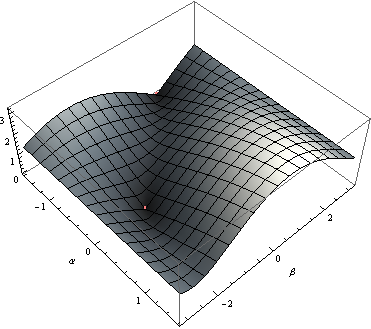
\includegraphics[width=0.8\textwidth]{figs/inversekinematics}
	\caption{Distance to $(x=1,y=1)$ over the configuration space of a two-arm manipulator. Minima corresponds to exact inverse kinematic solutions.}
	\label{fig:inversekinematics}
\end{figure}

You can now think about inverse kinematics as a path finding problem from anywhere in the configuration space to the nearest minima. A formal approach to doing this will be discussed in Section \ref{sec:advinvkinematics}. How to find shortest paths in space, that is finding the shortest route for a robot to get from A to B will be a subject of chapter \ref{chap:pathplanning}.
